\documentclass{article}
\usepackage{tikz}
\usepackage{geometry}
 \geometry{
 a4paper,
 total={170mm,257mm},
 left=20mm,
 top=20mm,
 }
\usetikzlibrary{arrows,shapes,positioning,shadows,trees}


\begin{document}

\begin{tikzpicture}
  \node (z) at (0,0) {
    \begin{tikzpicture}
      % fill space between the two circles
      \fill[gray!50,opacity=0.5] (0,0) circle (1) -- (1,0) circle (2.5);
      \fill[white] (0,0) circle (0.99);

      % draw circle centered at (0,0) radius 1, label \gamma_1
      \draw (0,0) circle (1);
      \node[anchor=north west] at (0.8,-0.6) {$\gamma_1$};
      % draw circle centered at (1,0) radius 5/2, label \gamma_2
      \draw (1,0) circle (2.5);
      \node[anchor=north west] at (1 + 2.5 * 0.8, 0 - 2.5 * 0.6) {$\gamma_2$};

      % label the origin
      \node[anchor=north east] at (0,0) {$O$};
      % label (1,0), (3.5,0)
      \node[anchor=south west] at (1,0) {$1$};
      \node[anchor=south west] at (3.5,0) {$\frac{7}{2}$};

      % label the space between the two circles as D
      \node[anchor=north west] at (1.5,2) {$D$};

      % label (-0.5, 0) z_1, (-1.0, 0) z_2 with dots
      \node[fill,circle,inner sep=1pt,label=above:$z_1$] at (-0.5,0) {};
      \node[fill,circle,inner sep=1pt,label=above:$z_2$] at (-2.0,0) {};

      % draw axis with no labels, size 4x4
      \draw[-] (-2,0) -- (4,0);
      \draw[-] (0,-3.5) -- (0,3.5);
    \end{tikzpicture}
  };

  \node (f) at (z.east) [anchor=west, xshift=1cm] {
    \begin{tikzpicture}
      \draw[->] (0,0) -- (2,0);

      % label it as f
      \node[anchor=south] at (1,0) {$f$};
    \end{tikzpicture}
  };

  \node (f_z) at (f.east) [anchor=west,xshift=1cm] {
    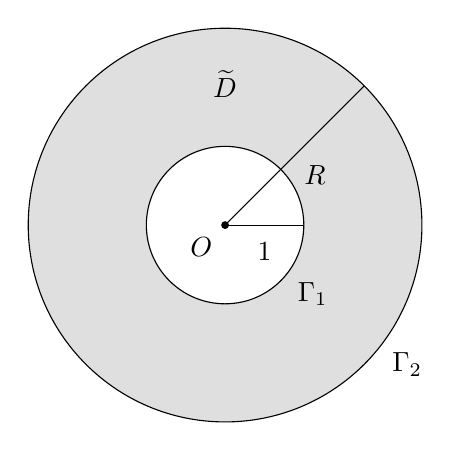
\begin{tikzpicture}

      % fill space between the two circles
      \fill[gray!50,opacity=0.5] (0,0) circle (1) -- (0,0) circle (2.5);
      \fill[white] (0,0) circle (0.99);

      % draw cicrle with radius 1, 2.5, centered at the origin, labeled as \Gamma_1, \Gamma_2
      \draw (0,0) circle (1);
      \node[anchor=north west] at (0.8,-0.6) {$\Gamma_1$};
      \draw (0,0) circle (2.5);
      \node[anchor=north west] at (0 + 2.5 * 0.8, 0 - 2.5 * 0.6) {$\Gamma_2$};

      % label (0,0) with a dot, captioned O at bottom left
      \node[fill,circle,inner sep=1pt,label=below left:$O$] at (0,0) {};

      % draw line from (0,0) to (1,0), label 1 under it's center, draw line from (0,0) with legth 2.5, pi/4 angle from the first line, label 2.5 under it's center
      \draw (0,0) -- (1,0);
      \node[anchor=north] at (0.5,-0.1) {$1$};
      \draw (0,0) -- (2.5 * 0.707, 2.5 * 0.707);
      \node[anchor=north west] at (2.5 * 0.707 / 2, 2.5 * 0.707 / 2) {$R$};

      \node[anchor=south] at (0,1.5) {$\widetilde{D}$};
    \end{tikzpicture}
  };
\end{tikzpicture}

\begin{tikzpicture}
  \node(z) at (0,0) {
    \begin{tikzpicture}
      % draw circle centered at (0,0) radius 1, label center at bottom with dot
      \draw (0,0) circle (1);
      \node[fill,circle,inner sep=1pt,label=below:$O$] at (0,0) {};
    \end{tikzpicture}
  };

  \node(f) at (z.east) [anchor=west, xshift=0.3cm] {
    \begin{tikzpicture}
      \draw[->] (0,0) -- (2,0);

      % label it as f
      \node[anchor=south] at (1,0) {$f$};
    \end{tikzpicture}
  };

  \node(f_z) at (f.east) [anchor=west, xshift=0.3cm] {
    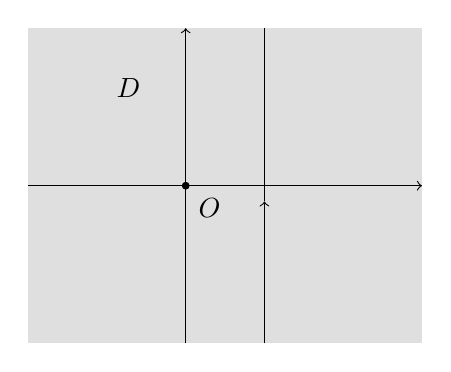
\begin{tikzpicture}
      % fill entire space with gray
      \fill[gray!50,opacity=0.5] (-2,-2) rectangle (3,2);

      \draw[->] (-2,0) -- (3,0);
      \draw[->] (0,-2) -- (0,2);

      % label origin with dot at bottom right
      \node[fill,circle,inner sep=1pt,label=below right:$O$] at (0,0) {};

      % label D at (-1, 1) up left
      \node[anchor=south west] at (-1,1) {$D$};

      % draw x=1 arrow pointing upwards
      \draw[->] (1,-2) -- (1,-0.2);
      \draw[-] (1,-0.2) -- (1,2);
    \end{tikzpicture}
  };

  \node(phi) at (f_z.south) [anchor=north, yshift=-0.3cm] {
    % same as f, but label it as \phi
    \begin{tikzpicture}
      \draw[->] (0,0) -- (0,-2);

      % label it as f
      \node[anchor=west] at (0,-1) {$\phi$};
    \end{tikzpicture}
  };

  \node(phi_f_z) at (phi.south) [anchor=north, yshift=-0.3cm] {
    % same as z
    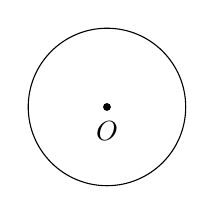
\begin{tikzpicture}
      % draw circle centered at (0,0) radius 1, label center at bottom with dot
      \draw (0,0) circle (1);
      \node[fill,circle,inner sep=1pt,label=below:$O$] at (0,0) {};
    \end{tikzpicture}
  };

  % connect z to phi_f_z
  \draw[->] (z) -- (phi_f_z);
\end{tikzpicture}
\end{document}